\paragraph{QuizziPedia::Front-End::Views::FillingQuestionnaireView}
\begin{figure} [ht]
	\centering
	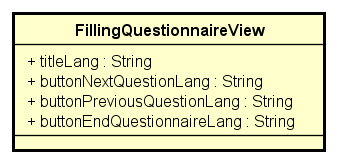
\includegraphics[scale=0.80]{UML/Classi/Front-End/QuizziPedia_Front-end_FillingQuestionnaireView.png}
	\caption{QuizziPedia::Front-End::Views:FillingQuestionnaireView}
\end{figure} \FloatBarrier
\begin{itemize}
	\item \textbf{Descrizione}: view principale per la compilazione del questionario; conterrà i vari templates di ogni domanda appartenente al questionario;
	\item \textbf{Utilizzo}: all'interno di essa verrà caricato inizialmente il template contenente le informazioni generali relative al questionario; verranno poi caricati i templates di ogni domanda presente nel questionario;
	\item \textbf{Relazioni con altre classi}: 
	\begin{itemize}
		\item \textit{IN} \texttt{FillingQuestionnaireController}: questa classe permette di gestire la compilazione del questionario;
		\item \textit{IN} \texttt{FillingQuestionnaireModelView}: classe di tipo modelview la cui istanzazione è contenuta all'interno della variabile di ambiente \$scope di \texttt{Angular.js}. All'interno di essa sono presenti le variabili e i metodi necessari per il \textit{Two-Way Data-Binding\ped{G}} tra la view \texttt{FillingQuestionnaireView} e il controller \texttt{FillingQuestionnaireController};
		\item \textit{IN} \texttt{InfoQuestionnaireDirective}: rappresenta il componente grafico che permette all'utente di visualizzare le informazioni principali del questionario che si sta per svolgere. Viene visualizzato dinamicamente all'interno delle views TrainingView e FillingQuestionnaireView mediante il controller QuestionsController;
		\item \textit{IN} \texttt{HeaderTextQuestionDirective}:rappresenta il componente grafico che presenta all'utente il testo della domanda, l'argomento e le parole chiave. Viene visualizzato dinamicamente all'interno delle views TrainingView e FillingQuestionnaireView mediante il controller QuestionsController;
		\item \textit{IN} \texttt{TrueFalseAnswerDirective}: rappresenta il componente grafico che permette all'utente di visualizzare la domanda vero e falso. Viene visualizzato dinamicamente all'interno delle views TrainingView e FillingQuestionnaireView mediante il controller QuestionsController;
		\item \textit{IN} \texttt{MultipleChoiceAnswerDirective}: rappresenta il componente grafico che permette all'utente di visualizzare la domanda a risposta multipla. Viene visualizzato dinamicamente all'interno delle views TrainingView e FillingQuestionnaireView mediante il controller QuestionsController;
		\item \textit{IN} \texttt{LinkingAnswerDirective}: rappresenta il componente grafico che permette all'utente di visualizzare la domanda di collegamento. Viene visualizzato dinamicamente all'interno delle views TrainingView e FillingQuestionnaireView mediante il controller QuestionsController;
		\item \textit{IN} \texttt{SortImagesAnswerDirective}: rappresenta il componente grafico che permette all'utente di visualizzare la domanda ad ordinamento di immagini. Viene visualizzato dinamicamente all'interno delle views TrainingView e FillingQuestionnaireView mediante il controller QuestionsController;
		\item \textit{IN} \texttt{SortTextAnswerDirective}: rappresenta il componente grafico che permette all'utente di visualizzare la domanda ad ordinamento di stringhe. Viene visualizzato dinamicamente all'interno delle views TrainingView e FillingQuestionnaireView mediante il controller QuestionsController;
		\item \textit{IN} \texttt{EmptySpaceAnswerDirective}: rappresenta il componente grafico che permette all'utente di visualizzare l'esercizio a riempimento di spazi vuoti. Viene visualizzato dinamicamente all'interno delle views TrainingView e FillingQuestionnaireView mediante il controller QuestionsController;
		\item \textit{IN} \texttt{ClickableAnswerDirective}: rappresenta il componente grafico che permette all'utente di visualizzare la domanda ad area cliccabile nell'immagine. Viene visualizzato dinamicamente all'interno delle views TrainingView e FillingQuestionnaireView mediante il controller QuestionsController;
		\item \textit{IN} \texttt{LangModel}: rappresenta il modello delle informazioni per la giusta traduzione dell'applicazione.
	\end{itemize}
		\item \textbf{Attributi}:
		\begin{itemize}
			\item \texttt{+ titleLang: String} \\ Attributo che viene utilizzato per visualizzare la giusta traduzione del titolo della pagina, in italiano o in inglese;
			\item \texttt{+ buttonNextQuestionLang: String} \\ Attributo che viene utilizzato per visualizzare la giusta traduzione della \textit{label\ped{G}} per il bottone di avanzamento a domanda successiva, in italiano o in inglese;
			\item \texttt{+ buttonPreviousQuestionLang: String} \\ Attributo che viene utilizzato per visualizzare la giusta traduzione della \textit{label\ped{G}} per il bottone di ritorno alla domanda precedente, in italiano o in inglese;
			\item \texttt{+ buttonEndQuestionnaireLang: String} \\ Attributo che viene utilizzato per visualizzare la giusta traduzione della \textit{label\ped{G}} per il bottone di conclusione del questionario, in italiano o in inglese. 
		\end{itemize}
\end{itemize}